\input ../SlidePreamble
\input ../preamble


\begin{document}

{\Huge

  \centerline{\bf TTIC 31230, Fundamentals of Deep Learning}
  \bigskip
  \centerline{David McAllester, Winter 2019}
  \vfill
  \centerline{Expectation Maximization (EM)}
  \vfill
  \centerline{The Evidence Lower Bound (the ELBO)}
  \vfill
  \centerline{Variational Autoencoders (VAEs)}
  \vfill
  \vfill

\slide{Latent Variable Models}

We are often interested in models of the form

\vfill
{\color{red} $$P_\Phi(y) = \sum_z\;P_\Phi(z)P_\Phi(y|z).$$}
{\color{red} $$P_\Phi(y|x) = \sum_z\;P_\Phi(z|x)P_\Phi(y|z).$$}

\vfill
For example, CTC and probabilistic grammar models.

\slidetwo{Expectation Maximization (EM)}
{Mixture of Gaussian Modeling}

{\color{red} $$\Phi = (\pi_1,\mu_1,\Sigma_1,\ldots,\pi_k,\mu_k,\Sigma_k)$$}

\begin{eqnarray*}
p_\Phi(y) & = & {\color{red} \sum_i\;P(i)P(y|i)} \\
\\
& = & \sum_i\;\pi_i\;\frac{1}{Z_i}\exp\left(-\frac{1}{2}(y-\mu_i)^\top \Sigma_i^{-1}(y - \mu_i)\right)
\end{eqnarray*}

\vfill
{\color{red} $i$ is the latent variable.}

\slidetwo{Expectation Maximization (EM)}
{Mixture of Gaussian Modeling}
\vspace{-4ex}
$$\Phi = (\pi_1,\mu_1,\Sigma_1,\ldots,\pi_k,\mu_k,\Sigma_k)$$
$$\mbox{Train} = \{y_1,\ldots,y_N\}$$
Until Convergence:
$$w[i,j] = P_\Phi(i|y_j) \;\;\mbox{\color{red} Inference (E step)}$$

$$\left.
\begin{array}{rcl}
  \pi_i & = & \frac{1}{N}\; \sum_j \;w[i,j] \\
  \mu_i & = & \frac{1}{N}\; \sum_j \;w[i,j]y_j \\
  \Sigma_i & = & \frac{1}{N}\; \sum_j w[i,j]y_jy_j^\top
\end{array}
  \right\} \mbox{\color{red} Model Update (M step)}$$

\slide{General EM}
{\color{red} $$\Phi^* = \argmin_\Phi E_{y \sim \mathrm{Train}} -\ln P_\Phi(y)$$}

\vfill
{\color{red} $$P_\Phi(y) = \sum_z\;P_\Phi(z)P_\Phi(y|z).$$}

\vfill
$${\color{red} \Phi^{t+1}} =  {\color{red} \argmin_\Phi}\;E_{y \sim \mathrm{Train}} \;E_{z \sim {\color{red} P_{\Phi^t}(z|y)}}\; - \ln P_{\color{red} \Phi}(z,y)$$
\centerline{M Step \hspace{6em} E Step \hspace{2.5em}~}
\centerline{\hspace{1em} Update \hspace{6em} Inference \hspace{2.5em}~}

\slide{Superpixel Colorization}

\centerline{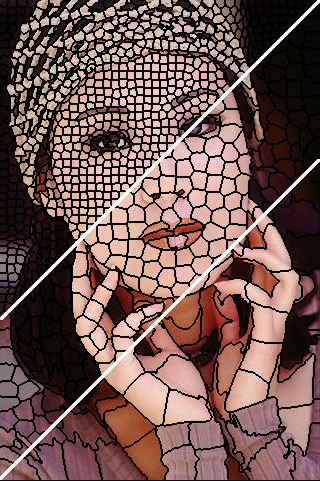
\includegraphics[height = 3in]{../images/SLIC} \hspace{.5in} 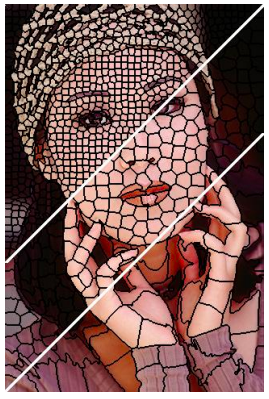
\includegraphics[height = 3in]{../images/SLICcolor}}
\centerline{\huge SLIC superpixels, Achanta et al.}

$x$ is a black and white image.

\vfill
$y$ is a color image drawn from $\pop(y|x)$.

\vfill
$\hat{y}$ is an arbitrary color image.

\vfill
$P_\Phi(\hat{y}|x)$ is the probability that model $\Phi$ assigns to the color image $\hat{y}$ given black and white image $x$.

\slideplain{Latent Semantic Segmentation (TZ)}

{\color{red} $$P_\Phi(y|x) = \sum_z\;P_\Phi(z|x)P_\Phi(y|z).$$}
\begin{eqnarray*}
\mbox{intput}\; x \\
P_\Phi(z|x) & = & \ldots \;\;\mbox{\color{red} semantic segmentation (friendly --- pixel RNN?)} \\
P_\Phi(\hat{y}|z) & = & \ldots \;\;\mbox{\color{red} colorization (friendly --- table lookup?)} \\
{\cal L}(y,\hat{y}) & = & -\ln\;p_\Phi(y|\hat{y}) \;\; \mbox{\color{red} distortion (friendly --- Gaussian)}
\end{eqnarray*}


\vfill
{\color{red} The composition is unfriendly.}

\slideplain{Maybe EM?}

\begin{eqnarray*}
\mbox{intput}\; x \\
P_\Phi(z|x) & = & \ldots \;\;\mbox{\color{red} semantic segmentation (friendly)} \\
P_\Phi(\hat{y}|z) & = & \ldots \;\;\mbox{\color{red} colorization (friendly)} \\
{\cal L}(y,\hat{y}) & = & -\ln\;p_\Phi(y|\hat{y}) \;\; \mbox{\color{red} distortion (friendly)}
\end{eqnarray*}

$${\color{red} \Phi^{t+1}} =  {\color{red} \argmin_\Phi}\;E_{y \sim \mathrm{Train}} \;E_{z \sim {\color{red} P_{\Phi^t}(z|y)}}\; - \ln P_{\color{red} \Phi}(z,y)$$
\centerline{\hspace{1em} Update \hspace{6em} Inference \hspace{2.5em}~}

\vfill
{\color{red} The inference is intractible!}

\slidetwo{Variational Inference:}
{The Evidence Lower Bound (The ELBO)}

$$P_\Phi(y) = \sum_z\;P_\Phi(z)P_\Phi(y|z)\;\;\mbox{\color{red} unfriendly composition of friendlies}$$
{\huge
\begin{eqnarray*}
\ln P_\Phi(y) & = & E_{\color{red} z \sim P_\Psi(z|y)} \ln P_\Phi(y) \;\;\;{\color{red} P_\Psi(z|y)\;\mbox{friendly}}\\
\\
 & = & E_{z \sim P_\Psi(z|y)} \left(\ln P_\Phi(y)P_\Phi(z|y) + \ln \frac{P_\Psi(z|y)}{P_\Phi(z|y)} + \ln\frac{1}{P_\Psi(z|y)}\right) \\
 \\
 & = & \left(E_{z \sim P_\Psi(z|y)} \;\ln\;P_\Phi(z,y)\right) + KL(P_\Psi(z|y),P_\Phi(z|y)) + H(P_\Psi(z|y)) \\
 \\
 & \geq & E_{\color{red} z \sim P_\Psi(z|y)}\;\left(\;\ln\;P_\Phi(z)P_\Phi(y|z) - \ln P_\Psi(z|y)\;\right) \;\;\;\mbox{\color{red} ELBO}
\end{eqnarray*}
}

\slidetwo{Variational Inference:}
{The Evidence Lower Bound (The ELBO)}

$$P_\Phi(y) = \sum_z\;P_\Phi(z)P_\Phi(y|z)\;\;\mbox{\color{red} unfriendly composition of friendlies}$$

\begin{eqnarray*}
\ln P_\Phi(y) & = & \mathrm{ELBO} + KL(P_\Psi(z|y),P_\Phi(z|y))
\end{eqnarray*}


\vfill
{\color{red} If the friendly $P_\Psi(z|y)$ can match the unfriendly $P_\Phi(z|y)$ then the ELBO is exact.}

\slide{Measuring the ELBO}

\vfill
{\color{red} $$\mathrm{ELBO}(y,\Phi,\Psi)  = E_{z\sim P_\Psi(y)} \; \ln P_\Phi(z)P_\Phi(y|z) - \ln P_\Psi(z)$$}

\vfill
If $P_\Phi(z)$, $P_\Phi(y|z)$, and $P_\Psi(z|y)$ are friendly (even whwn when $P_\Phi(y)$ is not friendly) we can
measure ELBO loss through sampling.

\vfill
If we can measure it, we can do gradient descent on it (but perhaps with difficulty).

\slide{Colorization}

\centerline{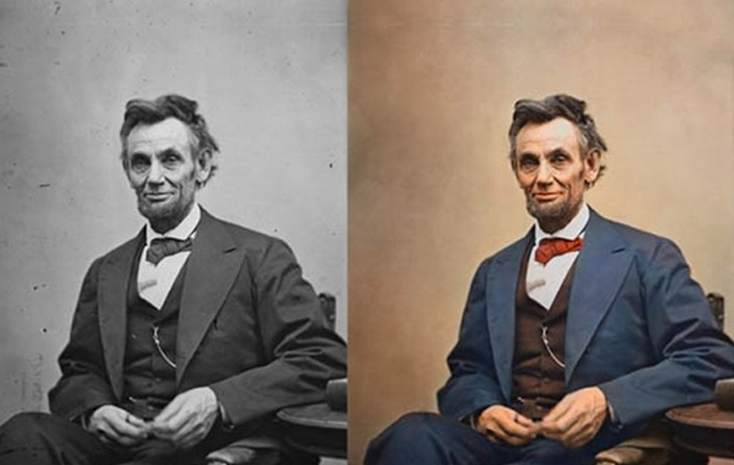
\includegraphics[height = 2in]{../images/Colorization}}

$x$ is a black and white image, $y$ a color image, and $z$ a semantic segmentation.

\vfill
$P_\Phi(z|x)$ is friendly and $P_\Phi(y|z,x)$ is friendly but $P(y|x)$ is not friendly.

\vfill
$P_\Psi(z|y,x)$ computes a friendly graphical model for $z$ given $y$.

\slide{A General ELBO Architecture}
\centerline{$P_\Phi(y|x)$ \hspace{10em} $P_\Psi(z|y,x)$}

\vfill
{\huge \color{red}
\parbox{4.0in}{
\begin{eqnarray*}
& & \mbox{intput}\; x \\
\vdots \\
z & = & \expsoftmax_z \ldots \\
\\
& & \mbox{input}\; z \\
\vdots \\
y & = & \expsoftmax_y\;\ldots
\end{eqnarray*}
}
\hfill
\parbox{4.0in}{
\begin{eqnarray*}
& & \mbox{intput}\; x,y \\
\vdots \\
z & = & \expsoftmax_z \ldots \\
\end{eqnarray*}
}
}
\vfill
The exponential softmaxes are friendly (they produce a friendly graphical model).

\slide{Two Expressions for the ELBO}

\begin{eqnarray*}
\ln P_\Phi(y) & = & ELBO(y,\Phi,\Psi) + KL(P_\Psi(z|y),P_\Phi(z|y)) \\
\\
 ELBO & = & E_{z \sim P_\Psi(z|y)}\; \ln P_\Phi(z,y) + H(P_\Psi(z|y))\;\;\;(1) \\
 \\      
  & = &{\color{red} \ln\;P_{\Phi}(y) - KL(P_\Psi(z|y),P_{\Phi}(z|y))\;\;\;\;\;\;(2)}
\end{eqnarray*}

\slide{EM is Alternating Maximization of the ELBO}
Forward-backward EM for HMMs and inside-outside EM for PCFGs (or any EM) can be written as

\vfill
\begin{eqnarray*}
\mathrm{\color{red} ELBO}& = & E_{z \sim P_\Psi(z|y)}\; \ln P_\Phi(z,y) + H(P_\Psi(z|y))\;\;\;(1) \\
 \\      
  & = & \ln\;P_{\Phi}(y) - KL(P_\Psi(z|y),P_{\Phi}(z|y))\;\;\;\;\;\;(2)
\end{eqnarray*}

\vfill
\begin{eqnarray*}
\mbox{by (2)}\;\;\;\Psi^{t+1} & = & \argmin_\Psi \;E_{y \sim \mathrm{Train}} \; KL(P_{\Psi}(z|y),P_{\Phi^t}(z|y)) {\color{red} = \Phi^t} \\
\\
\mbox{by (1)}\;\;\;{\color{red} \Phi^{t+1}} & = & \argmax_{\color{red} \Phi} E_{y \sim \mathrm{Train}} \;E_{z \sim P_{\color{red} {\Phi^t}}(z|y)}\; \ln P_{\color{red} \Phi}(z,y)
\end{eqnarray*}

\slide{We want $\Psi$ to adapt to $\Phi$}

$${\cal L}_{\mathrm{ELBO}}(y,\Phi,\Psi) = KL(P_\Psi(z|y),P_{\Phi}(z|y)) - \ln\;P_{\Phi}(y)$$

\vfill
$${\color{red} Q^*(z|y) = P_\Phi(z|y)}$$

\vfill
$$E_{y \sim \mathrm{Pop}}\;{\cal L}_{\mathrm{ELBO}}(y,\Phi,Q^*) = H(\mathrm{Pop},P_\Phi)$$

\slide{However, $\Phi$ can ignore $\Psi$}

$${\cal L}_{\mathrm{ELBO}}(y,\Phi,\Psi) = KL(P_\Psi(z|y),P_{\Phi}(z|y)) - \ln\;P_{\Phi}(y)$$

$${\color{red} P^*(z) = P_\Psi(z)}$$
$${\color{red} P^*(y|z) = P_\Phi(y)}$$

$$E_{y \sim \mathrm{Pop}}\;{\cal L}_{\mathrm{ELBO}}(y,P^*,\Psi) = H(\mathrm{Pop},P_\Phi)$$

\vfill
It seems important that $P_\Phi(y|z)$ have limited expressive power.

\slide{Hard ELBO}

Hard ELBO is to ELBO as hard EM is to EM.


\vfill
\begin{eqnarray*}
{\cal L}_{\mathrm{ELBO}}(y,\Phi,\Psi) &  =  & KL(P_\Psi(z|y),P_\Phi(z|y)) - \ln P_\Phi(y) \\
\\
{\cal L}_{\mathrm{ELBO}}(y,\Phi,\Psi) &  =  & E_{z \sim P_\Psi(z|y)} - \ln P_\Phi(z,y) + \ln P_\Psi(z|y) \\
\\
{\color{red} {\cal L}_{\mathrm{HELBO}}(y,\Phi,\Psi)} & {\color{red}  =} & {\color{red}  E_{z \sim P_\Psi(z|y)} - \ln P_\Phi(z,y)}
\end{eqnarray*}


\slide{Hard ELBO and Rate-Distortion Autoencoding}

\begin{eqnarray*}
{\cal L}_{\mathrm{HELBO}}(y,\Phi,\Psi) &  = &  E_{z \sim P_\Psi(z|y)} - \ln P_\Phi(z,y)
\end{eqnarray*}


\vfill
{\color{red} $$\min_{P,Q} E_{y \sim \mathrm{Pop}}\;{\cal L}_{\mathrm{HELBO}}(y,P,Q) \leq H(\mathrm{Pop}) + \ln 2$$}

\vfill
This can be proved from Shannon's source coding theorem where $z$ is the code for $y$.

\slide{A VAE for Images}

Auto-Encoding Variational Bayes, Diederik P Kingma, Max Welling, 2013.

\vfill
$${\color{red}y \hspace{5em}  z_\Psi(y,\epsilon) \hspace{4em} z\;p_\Phi(z) \hspace{3em} \hat{y}_\Phi(z) \hspace{3em}||y - \hat{y}||^2}$$
\centerline{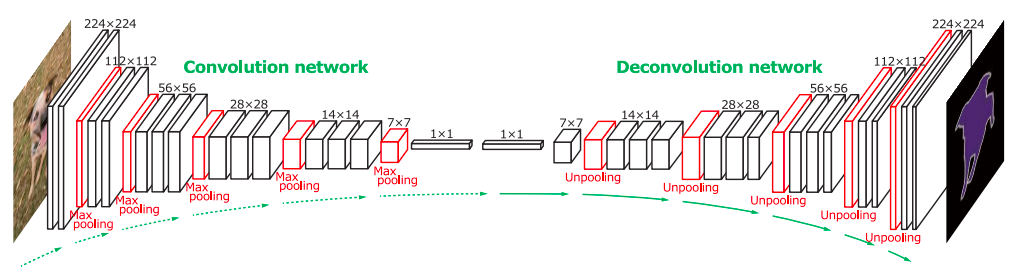
\includegraphics[width=9in]{../images/Deconv}}

\centerline{\Large [Hyeonwoo Noh et al.]}

\slide{Gaussian Distributions}

\begin{eqnarray*}
p_\Phi(z) & \propto & \exp\left(\sum_i \;(z[i] - {\color{red} \mu[i]})^2/(2{\color{red} \sigma[i]}^2)\right) \\
\\
p_\Phi(y|z) & \propto & \exp\left(\sum_j\;(y[j] - {\color{red} y_\Phi(z)[j]})^2/(2{\color{red} \gamma[j]}^2)\right) \\
\\
p_\Psi(z|y) & \propto & \exp\left(\sum_i (z[i] - {\color{red} z_\Psi(y)[i]})^2/(2{\color{red} \sigma_\Psi(y)[i]}^2)\right)
\end{eqnarray*}

\slide{KL-Divergence Form for the ELBO}

\begin{eqnarray*}
&  & E_{z \in p_\Psi(z|y)}\;\ln\;p_\Psi(z|y) - \ln\;p_\Phi(z)p_\Phi(y|z) \;\;\;\;{\color{red} {\cal L}_{\mathrm{ELBO}}} \\
\\
& = & {\color{red}  KL(p_\Psi(z|y),p_\Phi(z)) + E_{z \in P_\Psi(z|y)} - \ln p_\Phi(y|z)}
\end{eqnarray*}

\vfill
The ELBO is a KL-divergence + a cross entropy

\vfill
Continuous KL-divergence is ok.

\vfill
Continuous cross-entropy has issues --- we will come back to that
later.

\slide{Closed Form KL-Divergence}

\begin{eqnarray*}
& & KL(p_\Psi(z|y),p_\Phi(z)) \\
\\
\\
& = & \sum_i \;\frac{\sigma_\Psi(y)[i]^2 + (z_\Psi(y)[i]-\mu[i])^2}{2 \sigma[i]^2}
+ \ln\frac{\sigma[i]}{\sigma_\Psi(y)[i]} - \frac{1}{2}
\end{eqnarray*}


\slide{Standardizing $p_\Phi(z)$}

The KL-divergence term is
    
$$\sum_i \;\frac{{\color{red} \sigma}_\Psi(y)[i]^2 +({\color{red} z}_\Psi(y)[i] - {\color{red} \mu}[i])^2}{2 {\color{red} \sigma}[i]^2} + \ln\frac{{\color{red} \sigma}[i]}{{\color{red} \sigma}_\Psi(y)[i]} - \frac{1}{2}$$

\vfill
We can adjust $\Psi$ to $\Psi'$ such that
\begin{eqnarray*}
z_{\Psi'}(y)[i] & = & z_\Psi(y)[i]/\sigma[i] + \mu[i] \\
\sigma_{\Psi'}(y)[i] & = & \sigma_\Psi(y)/\sigma[i]
\end{eqnarray*}

\vfill
We then get {\color{red} $KL(p_{\Psi}(z|y),p_\Phi(z)) = KL(p_{\Psi'}(z|y),{\cal N}(0,I))$}.

\slide{Standardizing $p_\Phi(z)$}

\vfill
Without loss of generality the VAE becomes.

{\color{red} $$\min_{\Phi,\Psi}\; E_y\;KL(P_\Psi(z|y),{\cal N}(0,I)) + E_{z \in P_\Psi(z|y)} - \ln p_\Phi(y|z) $$}
\slide{Reparameterization Trick for the Cross-Entropy}

\begin{eqnarray*}
p_\Psi(z|y) & \propto & \exp\left(\sum_i (z[i] - {\color{red}
z_\Psi(y)[i]})^2/(2{\color{red} \sigma_\Psi(y)[i]}^2)\right)
\end{eqnarray*}

\vfill
\begin{eqnarray*}
& & E_{z \in p_\Psi(z|y)} \;\ln p_\Phi(y|z)\\
\\
\\
& = & E_{\epsilon \sim {\cal N}(0,I)} \;z[i] = {\color{red}
z_\Psi(y)[i]} + {\color{red} \sigma_\Psi(y)[i]}\epsilon[i];\;\; \;\ln
p_\Phi(y|z)
\end{eqnarray*}

\slide{Sampling}

$$P_\Psi(z|y) \hspace{3ex} z \hspace{3ex} P_\Phi(z,y)$$

\centerline{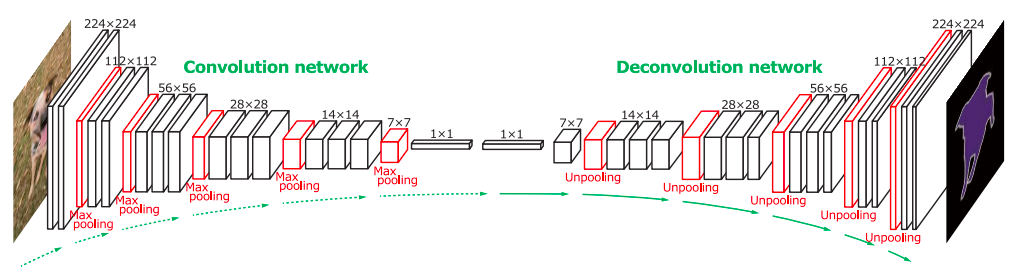
\includegraphics[width=6in]{../images/Deconv}}
\centerline{\large [Hyeonwoo Noh et al.]}

\vfill
Sampling uses just the second half ${\color{red} P_\Phi(z,y)}$.

\slide{Sampling}

\vfill
\centerline{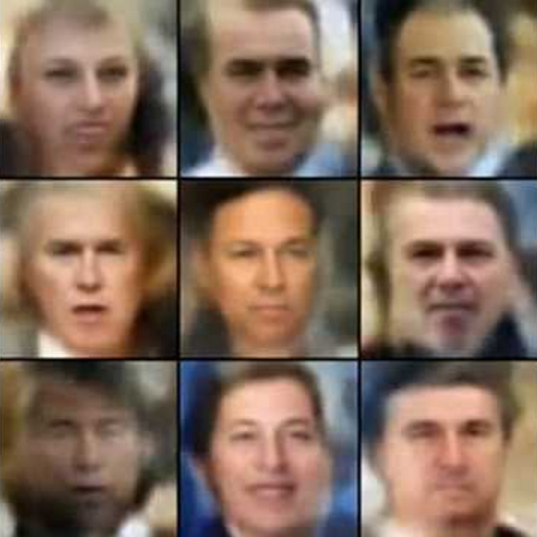
\includegraphics[width = 4in]{../images/VariationalFaces}}
\centerline{[Alec Radford]}

\slide{Why Blurry?}

A common explanation for the blurryness of images generated from VAEs
is the use of $L_2$ as the distortion measure.

\vfill
It does seem that $L_1$ works better.

\vfill
However, training on $L_2$ distortion can produce sharp images in
rate-distortion autoencoders.

\slide{Noisy-Channel Rate-Distortion Autoencoders}

\centerline{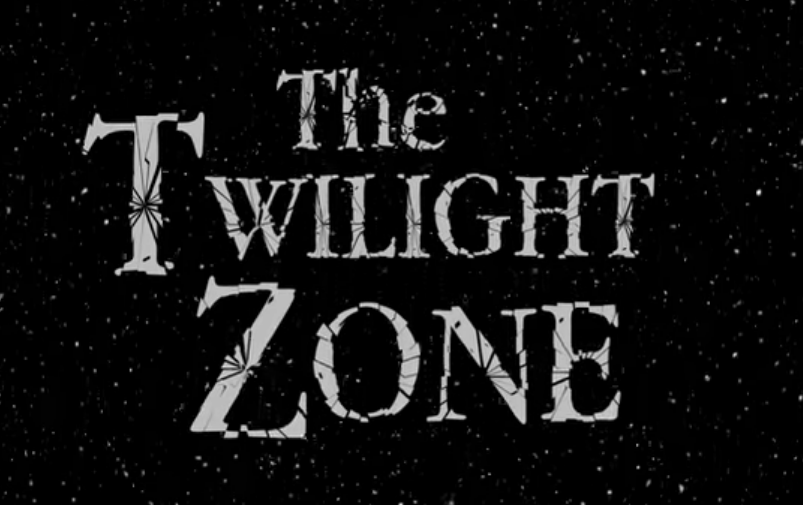
\includegraphics[width = 6in]{../images/Twilight}}

\vfill
The twilight zone is material for which I do not know of a reference. 

\slide{Differential Entropy and Cross-Entropy are Ill-Defined}

\bigskip
\begin{eqnarray*}
{\cal L}_{\mathrm{VAE}} & = & \sum_j\;\frac{E_{z \sim P_\Psi(z|y)}\;
({\color{red}y}[j] - {\color{red} \hat{y}}_\Phi(z)[j])^2}{2{\color{red} \gamma}[j]^2}
+ \ln {\color{red} \gamma}[j] \\
\\
& & + KL(p_\Psi(z|y),p_\Phi(z))
\end{eqnarray*}

\vfill Consider a probability density on light intensity.

\vfill
While the first term is dimensionless, ${\color{red} \gamma}[j]$ is an intensity.

\vfill
{\color{red} The cross-entropy term can be assigned any numerical value depending on the choice units (metric, English, or martian).}

\slide{Differential Entropy and Cross-Entropy are Ill-Defined}

There are also other problems with continuous entropy and cross-entropy.

\vfill
\begin{itemize}
\item Finite continuous entropy violates the source coding theorem --- it takes an infinite number of bits to code a real number.

\vfill
\item Finite continuous entropy violates the data processing inequality that $H(f(x)) \leq H(x)$.  For a continuous random variable $x$ under finite continuous entropy we can have $H(f(x)) > H(x)$.
\end{itemize}

\vfill
For these reasons it seems best to avoid using finite continuous entropy and finite continuous cross entropy.

\slide{Distortion}

A stochastic encoder $p_\Phi(z|y)$, a decoder $y_\Phi(z)$, and distortion function $D$ define a quantity of distortion.

$${\color{red} E_{y \sim \pop,\;z \sim p_\Phi(z|y)}\;D(y,y_\Phi(z))}$$

\vfill
For $L_2$ distortion we can use

$$D(y,y') = ||y - y'||_2$$

\vfill
Distortion can typically be given the same units as $y$.

\slide{Rate}

A stochastic encoder defines a rate.

\vfill
{\
\begin{eqnarray*}
p_\Phi(z) & \doteq & \sum_y\; \pop(y)p_\Phi(z|y) \\
\\
I_\Phi(y,z) & = &  E_y \;KL(p_\Phi(z|y),p_\Phi(z))
\end{eqnarray*}


\vfill
By Shannon's channel capacity theorem, $I_\Phi(y,z)$ is the channel capacity when sending $y$ across the noisy channel $z$.

\vfill
For $z$ continuous, a deterministic encoder has an infinite rate.

\vfill
{\color{red}  Here $p_\Phi(z)$ is not friendly.}

\slide{Bounding the Rate}

\begin{eqnarray*}
I_\Phi(y,z) & = & E_{y \sim \pop}\; KL(p_\Phi(z|y),p_\Phi(z)) \\
\\
& = & E_{y,z} \ln p_\Phi(z|y) - \ln p_\Psi(z) + \ln p_\Psi(z) - \ln p_\Phi(z) \\
\\
& = & E_y\;KL(p_\Phi(z|y),p_\Psi(z)) - KL(p_\Phi(z),p_\Psi(z)) \\
\\
& \leq & E_y\;KL(p_\Phi(z|y),p_\Psi(z))
\end{eqnarray*}

\vfill
{\color{red} We can take $p_\Psi(z)$ to be friendly, and WLOG, fixed at ${\cal N}(0,I)$.}

\slide{The Noisy-Channel Rate-Distortion Autoencoder}

{\color{red} {\Huge $$\Phi^* = \argmin_{\Phi}\;E_y \;KL(p_\Phi(z|y),{\cal N}(0,I)) \;+\; \frac{1}{\gamma} \; E_{z\sim p_\Phi(z|y)}\;D(y,\;y_\Phi(z))$$}}

\vfill
Here $\gamma$ has the same units as distortion and controls the trade-off between rate and distortion.

\slide{Summary: Rate-Distortion}


Rate-Distortion: $y$, continuous, $\tilde{z}$ a bit string,

{\color{red}
\begin{eqnarray*}
\Phi^* &  = &  \argmin_\Phi E_y \;|\tilde{z}_\Phi(y)| + \lambda D(y,y_\Phi(\tilde{z}_\Phi(y)))
\end{eqnarray*}
}

\vfill
Noisy Channel: {\color{red} $\tilde{z} = z_\Phi(y) + \sigma_\Phi(y) \odot \epsilon$,\hspace{2em} $\epsilon \sim {\cal N}(0,I)$}

{\color{red}
\begin{eqnarray*}
\Phi^* & = & \argmin_\Phi E_y\; \;KL(p_\Phi(\tilde{z}|y),{\cal N}(0,I)) + E_{\tilde{z}\sim p_\Phi(\tilde{z}|y)}\;\lambda D(y,y_\Phi(\tilde{z}))
\end{eqnarray*}
}

\slide{Summary: ELBO and VAE}


ELBO: {\color{red} $P_\Phi(z)$, $P_\Phi(y|z)$, $P_\Psi(z|y)$} friendly graphical models:

{\color{red} $$\Phi^*,\Psi^*  =  \argmin_{\Phi,\Psi}\; E_{y \sim \mathrm{Pop},\;z \sim P_\Psi(z|y)} \;\ln P_\Psi(z|y) - \ln P_\Phi(z)P_\Phi(y|z)$$}

\vfill
VAE: {\color{red} $p_\Phi(z|y)$, $p_\Phi(y|z)$} Gaussian:

{\color{red} $$\Phi^* =  \argmin_\Phi E_{y \sim \mathrm{Pop}}\; \;KL(p_\Phi(z|y),{\cal N}(0,I))  - E_{z\sim p_\Phi(z|y)}\;\ln p_\Phi(y|z)$$}

\slide{END}

}
\end{document}

